\documentclass[11pt,a4paper,twoside,openright]{article}

\title{Daftar Revisi Skripsi}
\author{Michael Adrian}

\usepackage{caption}
\usepackage{graphicx} 

\begin{document}

\maketitle

\begin{enumerate}
\item Halaman 49 baris 2, tertulis "2 kelas", seharusnya "3 kelas".
\item Halaman 64 baris 1 (baris 7 di buku), tertulis "GeneticParameterss", seharusnya "GeneticParameters"
\item Halaman 97, baris 11, seharusya tertulis "Lingkungan perangkat keras. Spesifikasi dari lingkungan ini dapat dilihat pada tabel 5.1."
\item Halaman 97, baris 13, seharusya tertulis "Lingkungan perangkat lunak. Spesifikasi dari lingkungan ini dapat dilihat pada tabel 5.2."
\item Halaman 115, tabel 5.6

Ukuran grid 4x4, rata-rata kecepatan tertulis 3.579 detik seharusnya 3.735 detik

\item Halaman 115, tabel 5.7

Ukuran grid 4x4, rata-rata kecepatan tertulis 4.002 detik seharusnya 4.183 detik

\item Halaman 115, tabel 5.8

Ukuran grid 4x4, rata-rata kecepatan tertulis 3.751 detik seharusnya 3.924 detik

\item Halaman 116, tabel 5.9

Ukuran grid 4x4, rata-rata kecepatan tertulis 4.175 detik seharusnya 4.371 detik

\item Halaman 116, tabel 5.10

Ukuran grid 4x4, rata-rata kecepatan tertulis 0.498 detik seharusnya 0.48 detik
Untuk grid 4x4, rata-rata tingkat keberhasilan tertulis 61.538\%, seharusnya 56.41\%

\item Halaman 116, tabel 5.11

Ukuran grid 4x4, rata-rata kecepatan tertulis 0.553 detik seharusnya 0.532 detik
Untuk grid 4x4, rata-rata tingkat keberhasilan tertulis 61.538\%, seharusnya 56.41\%

\item Halaman 117, tabel 5.12

Ukuran grid 4x4, rata-rata kecepatan tertulis 0.524 detik seharusnya 0.505 detik
Untuk grid 4x4, rata-rata tingkat keberhasilan tertulis 61.538\%, seharusnya 56.41\%

\item Halaman 117, tabel 5.13

Ukuran grid 4x4, rata-rata kecepatan tertulis 0.579 detik seharusnya 0.557 detik
Untuk grid 4x4, rata-rata tingkat keberhasilan tertulis 61.538\%, seharusnya 56.41\%

\item Halaman 117, tabel 5.14

Ukuran grid 4x4, rata-rata kecepatan tertulis 0.511 detik seharusnya 0.457 detik
Untuk grid 4x4, rata-rata tingkat keberhasilan tertulis 35.897\%, seharusnya 33.333\%

\item Halaman 118, tabel 5.15

Ukuran grid 4x4, rata-rata kecepatan tertulis 0.511 detik seharusnya 0.457 detik
Untuk grid 4x4, rata-rata tingkat keberhasilan tertulis 35.897\%, seharusnya 33.333\%

\item Halaman 118, tabel 5.16

Ukuran grid 4x4, rata-rata kecepatan tertulis 0.511 detik seharusnya 0.457 detik
Untuk grid 4x4, rata-rata tingkat keberhasilan tertulis 35.897\%, seharusnya 33.333\%

\item Halaman 118, tabel 5.17

Ukuran grid 4x4, rata-rata kecepatan tertulis 0.511 detik seharusnya 0.457 detik
Untuk grid 4x4, rata-rata tingkat keberhasilan tertulis 35.897\%, seharusnya 33.333\%

\item Halaman 118, tabel 5.18

Ukuran grid 4x4, rata-rata kecepatan tertulis 0.054 detik seharusnya 0.048 detik

\item Halaman 119, tabel 5.19

Ukuran grid 4x4, rata-rata kecepatan tertulis 0.054 detik seharusnya 0.048 detik

\item Halaman 119, tabel 5.20

Ukuran grid 4x4, rata-rata kecepatan tertulis 0.054 detik seharusnya 0.048 detik

\item Halaman 119, tabel 5.21

Ukuran grid 4x4, rata-rata kecepatan tertulis 0.054 detik seharusnya 0.048 detik

\item Halaman 145, tabel B.6

Baris 5 seharusnya 0.314 detik, 0.314 detik, 0.314 detik, dan 0.314 detik

Baris 7 seharusnya 4.905 detik, 5.517 detik, 5.211 detik, dan 5.823 detik

Baris 13 seharusnya 2.457 detik, 2.763 detik, 2.457 detik, dan 2.763 detik

Baris 16 seharusnya 0.62 detik, 0.62 detik, 0.62 detik, dan 0.62 detik

Baris 20 seharusnya 4.905 detik, 5.517 detik, 5.211 detik, dan 5.823 detik 

Baris 35 seharusnya 1.232 detik, 1.232 detik, 1.232 detik, dan 1.232 detik

\item Halaman 146, tabel B.7

Baris 5 seharusnya 0.063 detik, 0.063 detik, 0.063 detik, dan 0.063 detik

Baris 7 seharusnya Gagal, Gagal, Gagal, dan Gagal

Baris 13 seharusnya 0.999 detik, 1.109 detik, 1.054 detik, dan 1.164 detik

Baris 16 seharusnya 0.229 detik, 0.256 detik, 0.229 detik, dan 0.256 detik

Baris 20 seharusnya Gagal, Gagal, Gagal, dan Gagal

Baris 35 seharusnya 0.339 detik, 0.394 detik, 0.366 detik, dan 0.421 detik

\item Halaman 147, tabel B.8

Baris 5 seharusnya 0.314 detik, 0.314 detik, 0.314 detik, dan 0.314 detik

Baris 13 seharusnya Gagal, Gagal, Gagal, dan Gagal

Baris 16 seharusnya 0.62 detik, 0.62 detik, 0.62 detik, dan 0.62 detik

Baris 35 seharusnya 1.232 detik, 1.232 detik, 1.232 detik, dan 1.232 detik

Halaman 148, tabel B.9

Caption tertulis Skenario 5-8, seharusnya Skenario 13-16.

Baris 5 seharusnya 0.063 detik, 0.063 detik, 0.063 detik, dan 0.063 detik

Baris 35 seharusnya Gagal, Gagal, Gagal, dan Gagal

\item Setelah Lampiran B

Ada tambahan sebagai berikut:

Daftar jumlah sel yang berhasil diisi oleh algoritma \textit{rule based} untuk Calcudoku dengan ukuran \textit{grid} \begin{math}4 \times 4\end{math} dapat dilihat pada Tabel~\ref{tab:tabel1}.

\begin{table}
\centering
\captionsetup{justification=centering}
\caption[Daftar jumlah sel yang berhasil diisi oleh algoritma \textit{rule based} untuk Calcudoku dengan ukuran \textit{grid} \protect\begin{math}4 \times 4\protect\end{math}]{Daftar jumlah sel yang berhasil diisi oleh algoritma \textit{rule based} untuk Calcudoku dengan ukuran \textit{grid} \protect\begin{math}4 \times 4\protect\end{math}}
\begin{tabular}{| l | l |}
\hline
Nomor Soal & Jumlah Sel Diisi Algoritma \textit{Rule Based} \\
\hline \hline
1 & 0 \\
\hline
2 & 2 \\
\hline
3 & 0 \\
\hline
4 & 1 \\
\hline
5 & 6 \\
\hline
6 & 2 \\
\hline
7 & 1 \\
\hline
8 & 0 \\
\hline
9 & 9 \\
\hline
10 & 1 \\
\hline
11 & 1 \\
\hline
12 & 2 \\
\hline
13 & 2 \\
\hline
14 & 8 \\
\hline
15 & 0 \\
\hline
16 & 4 \\
\hline
17 & 3 \\
\hline
18 & 4 \\
\hline
19 & 1 \\
\hline
20 & 1 \\
\hline
21 & 2 \\
\hline
22 & 6 \\
\hline
23 & 0 \\
\hline
24 & 2 \\
\hline
25 & 16 \\
\hline
26 & 2 \\
\hline
27 & 1 \\
\hline
28 & 6 \\
\hline
29 & 2 \\
\hline
30 & 1 \\
\hline
31 & 0 \\
\hline
32 & 16 \\
\hline
33 & 0 \\
\hline
34 & 8 \\
\hline
35 & 3 \\
\hline
36 & 1 \\
\hline
37 & 2 \\
\hline
38 & 5 \\
\hline
39 & 1 \\
\hline
\end{tabular}
\label{tab:tabel1}
\end{table}

Daftar jumlah sel yang berhasil diisi oleh algoritma \textit{rule based} untuk Calcudoku dengan ukuran \textit{grid} \begin{math}5 \times 5\end{math} dapat dilihat pada Tabel~\ref{tab:tabel2}.

\begin{table}
\centering
\captionsetup{justification=centering}
\caption[Daftar jumlah sel yang berhasil diisi oleh algoritma \textit{rule based} untuk Calcudoku dengan ukuran \textit{grid} \protect\begin{math}5 \times 5\protect\end{math}]{Daftar jumlah sel yang berhasil diisi oleh algoritma \textit{rule based} untuk Calcudoku dengan ukuran \textit{grid} \protect\begin{math}5 \times 5\protect\end{math}}
\begin{tabular}{| l | l |}
\hline
Nomor Soal & Jumlah Sel Diisi Algoritma \textit{Rule Based} \\
\hline \hline
1 & 4 \\
\hline
2 & 0 \\
\hline
3 & 15 \\
\hline
4 & 1 \\
\hline
5 & 1 \\
\hline
6 & 1 \\
\hline
7 & 5 \\
\hline
8 & 1 \\
\hline
9 & 5 \\
\hline
10 & 0 \\
\hline
11 & 0 \\
\hline
12 & 3 \\
\hline
13 & 15 \\
\hline
14 & 2 \\
\hline
15 & 0 \\
\hline
16 & 1 \\
\hline
17 & 0 \\
\hline
18 & 16 \\
\hline
19 & 4 \\
\hline
20 & 2 \\
\hline
21 & 8 \\
\hline
22 & 14 \\
\hline
23 & 1 \\
\hline
24 & 5 \\
\hline
25 & 5 \\
\hline
26 & 1 \\
\hline
\end{tabular}
\label{tab:tabel2}
\end{table}

\item Poster

Pada bagian Hasil Pengujian, hasil pengujian untuk algoritma \textit{hybrid genetic} yang benar ditampilkan pada Gambar~\ref{fig:gambar1}.

\begin{figure}
\centering
\captionsetup{justification=centering}
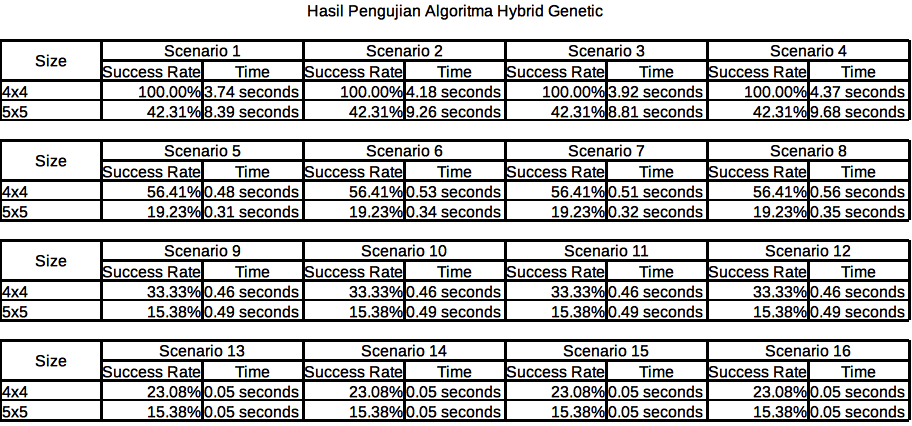
\includegraphics[scale=0.5]{HasilPengujianHG.png}
\caption[Hasil pengujian algoritma \textit{hybrid genetic}]{Hasil pengujian algoritma \textit{hybrid genetic}}
\label{fig:gambar1}
\end{figure}

\end{enumerate}

\end{document}